%% ============================================================
%% TRIsecure: Design and Evaluation of a Three-Factor Post-Quantum
%% Biometric E-Voting Framework on Commodity Edge Hardware
%%
%% Journal : Information and Computer Security (ICS), Emerald Publishing
%%
%% COMPILE: pdfLaTeX -> BibTeX -> pdfLaTeX -> pdfLaTeX
%% Overleaf: Compiler = pdfLaTeX  |  Bibliography = BibTeX
%% ============================================================

\documentclass[a4paper,12pt]{article}

%% -- Geometry and encoding ------------------------------------
\usepackage[top=2.5cm,bottom=2.5cm,left=3cm,right=3cm]{geometry}
\usepackage[T1]{fontenc}
\usepackage[utf8]{inputenc}

%% -- Mathematics ----------------------------------------------
\usepackage{amsmath,amssymb}

%% -- Figures --------------------------------------------------
\usepackage{graphicx}

%% -- Tables ---------------------------------------------------
\usepackage{booktabs}

%% -- Bibliography (natbib + bibtex, no biber) ----------------
\usepackage[round,authoryear,sort&compress]{natbib}
\usepackage{url}

%% -- Section headings: Emerald style (no titlesec) -----------
%% H1: large bold  |  H2+H3: normalsize italic
\makeatletter
\renewcommand\section{\@startsection{section}{1}{\z@}%
  {-14pt \@plus -4pt \@minus -2pt}{6pt \@plus 2pt}%
  {\normalfont\large\bfseries}}
\renewcommand\subsection{\@startsection{subsection}{2}{\z@}%
  {-10pt \@plus -3pt \@minus -2pt}{4pt \@plus 2pt}%
  {\normalfont\normalsize\itshape}}
\renewcommand\subsubsection{\@startsection{subsubsection}{3}{\z@}%
  {-8pt \@plus -2pt}{3pt \@plus 1pt}%
  {\normalfont\normalsize\itshape}}
\makeatother

%% -- Theorem environments ------------------------------------
\newtheorem{theorem}{Theorem}
\newtheorem{definition}{Definition}

%% -- Emerald: Roman-numeral table numbering ------------------
\renewcommand{\thetable}{\Roman{table}}

%% -- Citation aliases ----------------------------------------
\newcommand{\parencite}[1]{\citep{#1}}
\newcommand{\textcite}[1]{\citet{#1}}

%% -- booktabs alias ------------------------------------------
\newcommand{\botrule}{\bottomrule}

%% -- Spacing tweaks ------------------------------------------
\setlength{\emergencystretch}{4em}
\setlength{\tolerance}{1500}
\setlength{\parskip}{6pt}
\setlength{\parindent}{0pt}

\bibliographystyle{apalike}

%% =============================================================
\begin{document}
%% =============================================================

%% BLIND SUBMISSION: author block withheld for peer review.
%% Add all authors via ScholarOne at submission.
%% Uncomment \author block below ONLY for the final accepted version.
\title{\textbf{TRIsecure: Design and Evaluation of a Three-Factor
  Post-Quantum Biometric E-Voting Framework on Commodity Edge Hardware}}
\author{}        % left blank for blind review
%% \author{Pinnemcharla Sai Vivek Reddy$^{1*}$,
%%   Saranya G$^{1}$ and S.\ Udhaya Kumar$^{1}$\\[6pt]
%%   $^{1}$Department of Computer Science and Engineering,\\
%%   Amrita Vishwa Vidyapeetham, Chennai, Tamil Nadu, India\\[4pt]
%%   $^{*}$Corresponding author.
%%   E-mail: \texttt{vivekreddy9036@gmail.com}\\
%%   Contributing authors:
%%   \texttt{g\_saranya@ch.amrita.edu};
%%   \texttt{u\_udhayakumar@ch.amrita.edu}}
\date{}
\maketitle
\thispagestyle{empty}

%% -------------------------------------------------------------
%% STRUCTURED ABSTRACT (Emerald format, max 250 words)
%% -------------------------------------------------------------
\begin{abstract}
\noindent\textbf{Purpose} --
Electronic voting systems must simultaneously satisfy strong voter
authentication, tamper-evident vote integrity, end-to-end voter
verifiability, and practical deployment on resource-limited hardware.
This paper presents TRIsecure V2, a three-factor biometric e-voting
terminal designed to jointly satisfy all four requirements on commodity
Raspberry Pi~4 (ARM64) hardware without server-grade infrastructure or
persistent cloud connectivity.

\medskip\noindent\textbf{Design/methodology/approach} --
TRIsecure V2 integrates an ISO/IEC~19795-1 compliant biometric pipeline
with Bayesian score-level fusion of face recognition and NFC card
modalities, ISO/IEC~30107-3 presentation attack detection (MiniFASNetV2
liveness), a hybrid post-quantum cryptographic layer (Kyber-768\,+\,X25519
KEM and Dilithium-3\,+\,Ed25519 signatures per NIST FIPS~203/204), and a
formally verified five-stage authentication protocol modelled as a
Deterministic Finite Automaton (DFA) with six proved security properties.

\medskip\noindent\textbf{Findings} --
Simulation-based evaluation following ISO/IEC~19795-6 achieves
EER\,=\,1.55\%, AUC\,=\,0.9991, TAR@1\%FAR\,=\,97.7\% and
ACER\,=\,4.25\%. On-device benchmarking demonstrates 110.7\,ms
end-to-end authentication latency (p99\,=\,111.3\,ms) and
541.6~voters/min throughput. Bayesian NFC\,+\,face fusion reduces the
effective combined-attack false accept rate by three orders of magnitude
relative to face-only authentication.

\medskip\noindent\textbf{Originality/value} --
To the best of the authors' knowledge, this is the first e-voting system
to simultaneously provide formal protocol verification, post-quantum
cryptography, liveness detection, and end-to-end verifiability on
low-cost edge hardware, confirming feasibility for small-to-medium
polling station deployment.

\medskip\noindent\textbf{Keywords:} biometric authentication, e-voting,
formal verification, post-quantum cryptography, edge computing,
presentation attack detection, Bayesian fusion, Merkle proof, liveness
detection, NFC authentication

\medskip\noindent\textbf{Article Classification:} Research paper
\end{abstract}

\newpage\setcounter{page}{1}

%% =============================================================
\section{Introduction}\label{sec:intro}
%% =============================================================

\subsection{Background}

Electronic voting systems are critical infrastructure where failure
consequences are asymmetric: a single undetected fraud vector can undermine
election legitimacy at scale. The fundamental security challenge is to
authenticate the right voter, record the right vote, prevent tampering, and
allow the voter to verify their participation---all while running on
deployable, affordable hardware.

\subsection{Problem Statement}

Existing systems leave at least one of these requirements unsatisfied.
Fingerprint- and face-based voting systems
\parencite{bello2021biometric,sanchez2020biometric,komatineni2020biometric,nagaraj2022voting}
report biometric error rates without formal protocol verification or
post-quantum (PQC) readiness. Blockchain-based approaches
\parencite{ayed2017conceptual,hardwick2018voting,faruk2024transforming}
provide strong vote integrity but lack biometric authentication and rely on
classical cryptography vulnerable to quantum adversaries
\parencite{bernstein2017post}; a comprehensive review of 81~blockchain
voting systems by \textcite{huang2022blockchain_voting} confirms this gap.
Industry multi-factor authentication standards (FIDO2/WebAuthn)
\parencite{fido2_webauthn} are not designed for the one-time-per-election
voting constraint and incorporate neither formal liveness detection nor
voter-verifiable receipts. None of the above have been formally verified
at the protocol level.

\subsection{Research Gap}

No existing e-voting system jointly provides: (i)~multi-factor biometric
authentication with liveness detection, (ii)~formally verified protocol
security, (iii)~post-quantum cryptographic readiness, and
(iv)~end-to-end voter verifiability---all on low-cost edge hardware
without server infrastructure.

\subsection{Objectives}

This work aims to:
\begin{itemize}
  \item Design and implement a three-factor biometric e-voting terminal
        deployable on Raspberry Pi~4 (ARM64) hardware.
  \item Formally verify the authentication protocol's security properties
        using automata-theoretic methods.
  \item Integrate hybrid post-quantum cryptography to provide a
        quantum-resistance transition path.
  \item Provide end-to-end voter verifiability through cryptographic
        receipts and Merkle inclusion proofs.
\end{itemize}

\subsection{Contributions}

The following original contributions are made:

\renewcommand{\labelenumi}{\textbf{C\arabic{enumi}.}}
\begin{enumerate}
  \item \textbf{Formally verified multi-factor authentication.}
        A five-stage pipeline modelled as a DFA with six proved security
        properties: determinism, completeness, safety, liveness,
        double-vote prevention, and rate-limit enforcement.
  \item \textbf{Bayesian score-level biometric fusion.}
        Log-likelihood-ratio fusion of face cosine similarity and NFC
        channel evidence (EER\,=\,1.55\%, AUC\,=\,0.9991,
        TAR@1\%FAR\,=\,97.7\%).
  \item \textbf{Hybrid post-quantum cryptographic layer.}
        Kyber-768\,+\,X25519 hybrid KEM (NIST FIPS~203) and
        Dilithium-3\,+\,Ed25519 digital signatures (NIST FIPS~204).
  \item \textbf{ISO/IEC~30107-3 presentation attack detection.}
        MiniFASNetV2 liveness detection integrated at the final
        authentication stage (BPCER\,=\,1.0\%, ACER\,=\,4.25\%).
  \item \textbf{End-to-end voter verifiability.}
        SHA-256 commitment receipts and $O(\log n)$ Merkle inclusion
        proofs.
  \item \textbf{Edge-device evaluation.}
        Full-system benchmarks on Raspberry Pi~4 (ARM64): 110.7\,ms
        end-to-end latency (p99\,=\,111.3\,ms), 541.6~voters/min
        throughput.
\end{enumerate}
\renewcommand{\labelenumi}{\arabic{enumi}.}

\subsection{Novelty Discussion}

No individual component is claimed as algorithmically novel in isolation:
DFA-based verification, Bayesian score-level fusion, hybrid PQC,
lightweight CNN liveness detection, and Merkle-proof vote receipts each
have independent prior literature. The novel contribution is their
\emph{principled co-design} within a single formally verified pipeline
running on low-cost edge hardware. To the best of the authors' knowledge,
no prior e-voting system has jointly delivered formal protocol
verification, quantum-resistant cryptography, ISO/IEC~30107-3 liveness
detection, and voter-verifiable receipts within a single commodity device.

The remainder of this paper is organised as follows.
Section~\ref{sec:related} surveys related work.
Section~\ref{sec:architecture} describes the system architecture.
Section~\ref{sec:security} presents the formal security analysis.
Section~\ref{sec:evaluation} reports experimental results.
Section~\ref{sec:discussion} discusses findings and limitations.
Section~\ref{sec:conclusion} concludes.

%% =============================================================
\section{Related Work}\label{sec:related}
%% =============================================================

\subsection{Biometric E-Voting Systems}

\textcite{bello2021biometric} propose a fingerprint-and-smart-card voting
system achieving EER\,=\,2.5\% with 950\,ms authentication latency.
\textcite{sanchez2020biometric} examine biometric verification in
constrained environments (EER\,=\,3.2\%, 480\,ms).
\textcite{komatineni2020biometric} combine machine learning-based face
detection with biometric scanning for duplicate-vote prevention.
\textcite{nagaraj2022voting} integrate facial recognition with fingerprint
authentication. \textcite{revathy2022cnn_evoting} combine CNN-based face
recognition with blockchain and blind signatures.
\textcite{faruk2024transforming} deploy blockchain and biometric
verification over Hyperledger Fabric (87\% biometric registration success
across 100 participants) but rely on classical cryptography with no formal
protocol verification. None of these systems incorporate formal
automata-theoretic protocol verification, post-quantum cryptographic
readiness, or ISO/IEC~30107-3 compliant liveness detection.

\subsection{Blockchain-Based Voting}

\textcite{ayed2017conceptual} proposes an Ethereum-based system with
blockchain receipts but PIN-only authentication.
\textcite{hardwick2018voting} extend this with anonymisation techniques;
\textcite{hjalmarsson2018blockchain} demonstrate a Hyperledger Fabric
deployment. \textcite{huang2022blockchain_voting} survey 81~blockchain
voting works, identifying decentralisation and integrity as primary design
axes while noting voter authentication and anti-spoofing as open problems.
\textcite{hajian2024blockchain} confirm biometric identity binding is
absent from current blockchain e-voting deployments.

\subsection{Post-Quantum Cryptography on Edge Hardware}

\textcite{sikeridis2020pqc} evaluate PQC algorithms in TLS~1.3 on
constrained ARM hardware, showing Kyber-768 and Dilithium-3 to be
feasible with the \texttt{liboqs} library. NIST finalised ML-KEM
(Kyber-768, FIPS~203) \parencite{nist_fips203} and ML-DSA (Dilithium-3,
FIPS~204) \parencite{nist_fips204} in 2024.
\textcite{paquin2019oqs} benchmark the Open Quantum Safe library across
ARM platforms; \textcite{kannwischer2019pqm4} characterise PQC on
Cortex-M4.

\subsection{Presentation Attack Detection}

ISO/IEC~30107-3 \parencite{iso30107} defines the standard PAD evaluation
framework specifying APCER, BPCER, and ACER metrics.
\textcite{zhang2020minifasnet} introduce MiniFASNetV2, a lightweight CNN
suitable for embedded deployment. Complementary PAD approaches include
depth-based auxiliary supervision \parencite{liu2018learning}, spoof-noise
disentanglement \parencite{jourabloo2018desp}, and spectral artefact
analysis \parencite{zhang2019autoGAN}. Benchmark datasets include NUAA
\parencite{tan2010nuaa} and OULU-NPU \parencite{boulkenafet2017oulu}.
\textcite{yang2023pad_survey} confirm lightweight CNN models remain
competitive under deployment computational constraints.

\subsection{Formal Verification and E-Voting Verifiability}

ProVerif \parencite{blanchet2016proverif} and Tamarin
\parencite{meier2013tamarin} are standard symbolic protocol analysis tools.
Automata-theoretic verification is preferred in this work because the
security properties concern pipeline control-flow (ordering, completeness,
determinism, termination) rather than cryptographic secrecy goals.
Cryptographic e-voting work---including Helios \parencite{adida2008helios},
Civitas \parencite{clarkson2008civitas}, and Scantegrity~II
\parencite{chaum2009scantegrity}---provides strong verifiability but lacks
biometric authentication.

\subsection{Multimodal Biometric Fusion}

\textcite{ross2003multimodal} establish the taxonomy of biometric fusion
levels. \textcite{nandakumar2008fusion} derive optimal likelihood-ratio
score fusion under Gaussian density estimation, the approach adopted in
this work. \textcite{fierrez2005fusion} extend this with quality-based
weighting; \textcite{jain2011multimodal} provide a comprehensive
multimodal survey.

\subsection{Comparison with Prior Work}

Table~\ref{tab:related_comparison} summarises reference systems against
TRIsecure V2 across key capability axes.

\begin{table}[htbp]
\caption{Comparison of related e-voting and biometric authentication
  systems. PAD\,=\,presentation attack detection;
  PQC\,=\,post-quantum cryptography; FV\,=\,formal verification;
  BIO\,=\,biometric.}
\label{tab:related_comparison}
\small
\begin{tabular}{p{2.5cm}p{3.0cm}p{3.9cm}p{3.1cm}}
  \toprule
  \textbf{Author (Year)} & \textbf{Method} &
  \textbf{Advantages} & \textbf{Limitations} \\
  \midrule
  \textcite{bello2021biometric}
    & Fingerprint + smart card
    & Two-factor BIO; EER 2.5\%
    & No PAD; no PQC; no FV \\[2pt]
  \textcite{sanchez2020biometric}
    & Face + smart card, embedded
    & Constrained; two-factor
    & EER 3.2\%; no liveness; no FV \\[2pt]
  \textcite{ayed2017conceptual}
    & Ethereum, PIN-only
    & Blockchain receipts
    & No BIO; classical crypto \\[2pt]
  \textcite{faruk2024transforming}
    & Hyperledger + face + fingerprint
    & Dual-BIO; blockchain
    & No PAD; no PQC; no FV \\[2pt]
  \citet{fido2_webauthn}
    & Device-bound MFA standard
    & Industry standard; keys
    & No PAD; no voter receipts \\[2pt]
  \textbf{TRIsecure V2}
    & NFC+face+token; PAD; PQC; DFA
    & Formally verified; PAD; PQC; edge
    & Simulation BIO; no field trial \\
  \botrule
\end{tabular}
\end{table}

%% =============================================================
\section{System Architecture}\label{sec:architecture}
%% =============================================================

\subsection{Design Goals and Threat Model}

TRIsecure V2 is designed to satisfy five security and operational goals:

\begin{description}
  \item[\textbf{G1 -- Authentication.}] Each vote is bound to exactly one
    registered voter, verified via three independent factors.
  \item[\textbf{G2 -- Vote integrity.}] Vote records are tamper-evident
    and auditable by any external party.
  \item[\textbf{G3 -- Voter privacy.}] Face embeddings are encrypted at
    rest; vote--voter linkage is separated in the database schema.
  \item[\textbf{G4 -- Verifiability.}] Voters can confirm their vote was
    recorded; auditors can verify the tally without accessing individual
    votes.
  \item[\textbf{G5 -- Edge viability.}] The full system runs on commodity
    ARM64 hardware within 200\,ms end-to-end latency.
\end{description}

The threat model covers four adversary categories: (1)~\textbf{remote
attacker} (brute-force, replay, man-in-the-middle); (2)~\textbf{physical
attacker} (spoofed face photo or video, cloned NFC card);
(3)~\textbf{insider attacker} (database read/write access but no
biometric secret or NFC card); (4)~\textbf{quantum adversary} (capable
of breaking RSA/ECC via Shor's algorithm \parencite{shor1994algorithms}).

\subsection{System Overview}

Figure~1 shows the six-layer clean architecture. A voter interaction
proceeds as: (1)~tap NFC card at PN532 reader; (2)~live face capture by
camera; (3)~Bayesian fusion evaluates combined NFC\,+\,face
log-likelihood ratio; (4)~MiniFASNetV2 PAD liveness check; (5)~one-time
session token issued (60\,s TTL); (6)~ballot selection; (7)~vote recorded
to SHA-256 hash chain; (8)~Merkle receipt generated and saved.

\begin{figure}[htbp]
  \centering
  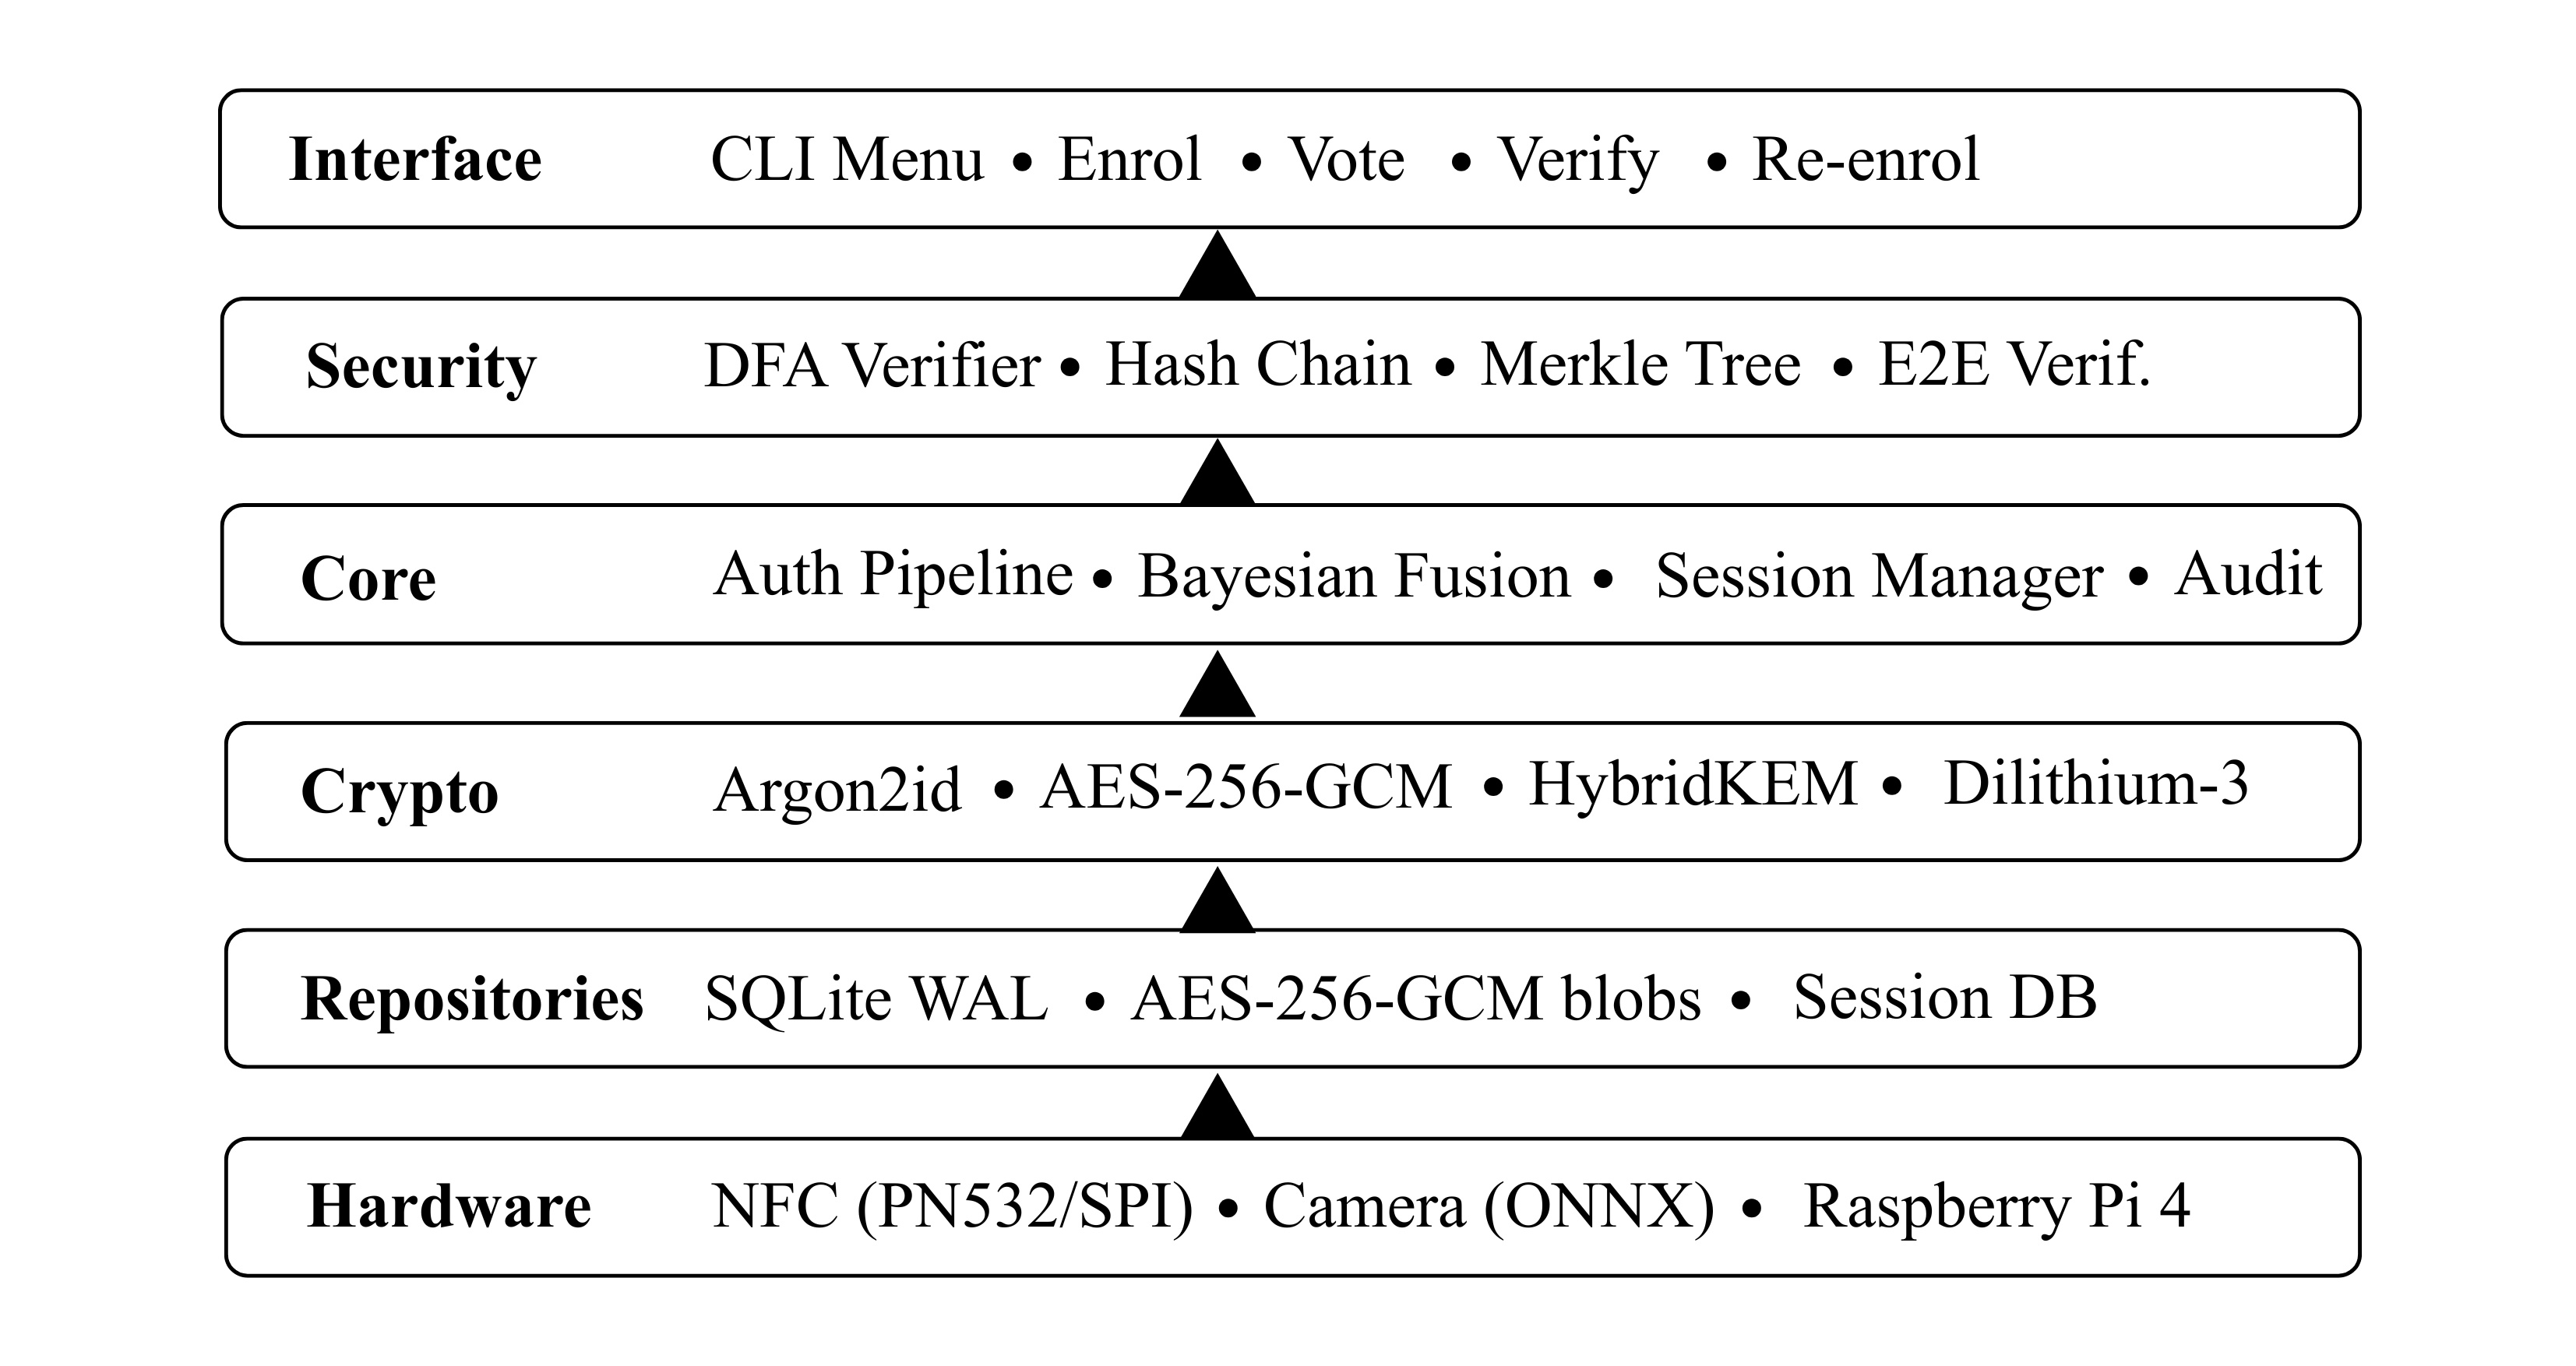
\includegraphics[width=\linewidth]{figures/architecture.jpg}
  \caption{TRIsecure V2 six-layer clean architecture. Arrows show upward
    dependency direction; hardware details are abstracted at each layer
    boundary.}
  \label{fig:architecture}
\end{figure}

\subsection{Multi-Factor Authentication Pipeline}\label{sec:pipeline}

The authentication pipeline is a five-stage sequential process formally
modelled as a DFA $\mathcal{M} = (Q, \Sigma, \delta, q_0, F)$
(Section~\ref{sec:dfa}). Figure~2 shows the state diagram. The pipeline
enforces strict ordering: no stage is attempted before the previous
stage succeeds; any failure transitions deterministically to
\textsc{Rejected}.

\paragraph{Stage~1 -- Rate limiting.}
A sliding-window counter per NFC~UID (5 failures per 300\,s) blocks
brute-force before any biometric computation.

\paragraph{Stage~2 -- NFC verification.}
The PN532 SPI reader captures the voter's NFC~UID
\parencite{hasan2019nfc}, validated against the encrypted voter database
with AES-256-GCM encrypted session binding.

\paragraph{Stage~3 -- Voter eligibility.}
The \texttt{has\_voted} flag is atomically checked;
\texttt{NOT\_ELIGIBLE} immediately transitions to \textsc{Rejected}
(DFA property~P5, double-vote prevention).

\paragraph{Stage~4 -- Bayesian score-level fusion.}
Face cosine similarity (ArcFace MobileFaceNet embedding, 512-D) and NFC
channel evidence are combined via log-likelihood ratio fusion
(Section~\ref{sec:fusion}).

\paragraph{Stage~5 -- Presentation attack detection.}
MiniFASNetV2 classifies the captured face frame as live or spoofed.
\texttt{PAD\_ATTACK} transitions to \textsc{Rejected}.

\paragraph{Session issuance.}
A 256-bit cryptographically random session token with 60\,s TTL is
issued. Only the SHA-256 hash of the token is stored to prevent
token-exposure attacks.

\begin{figure}[htbp]
  \centering
  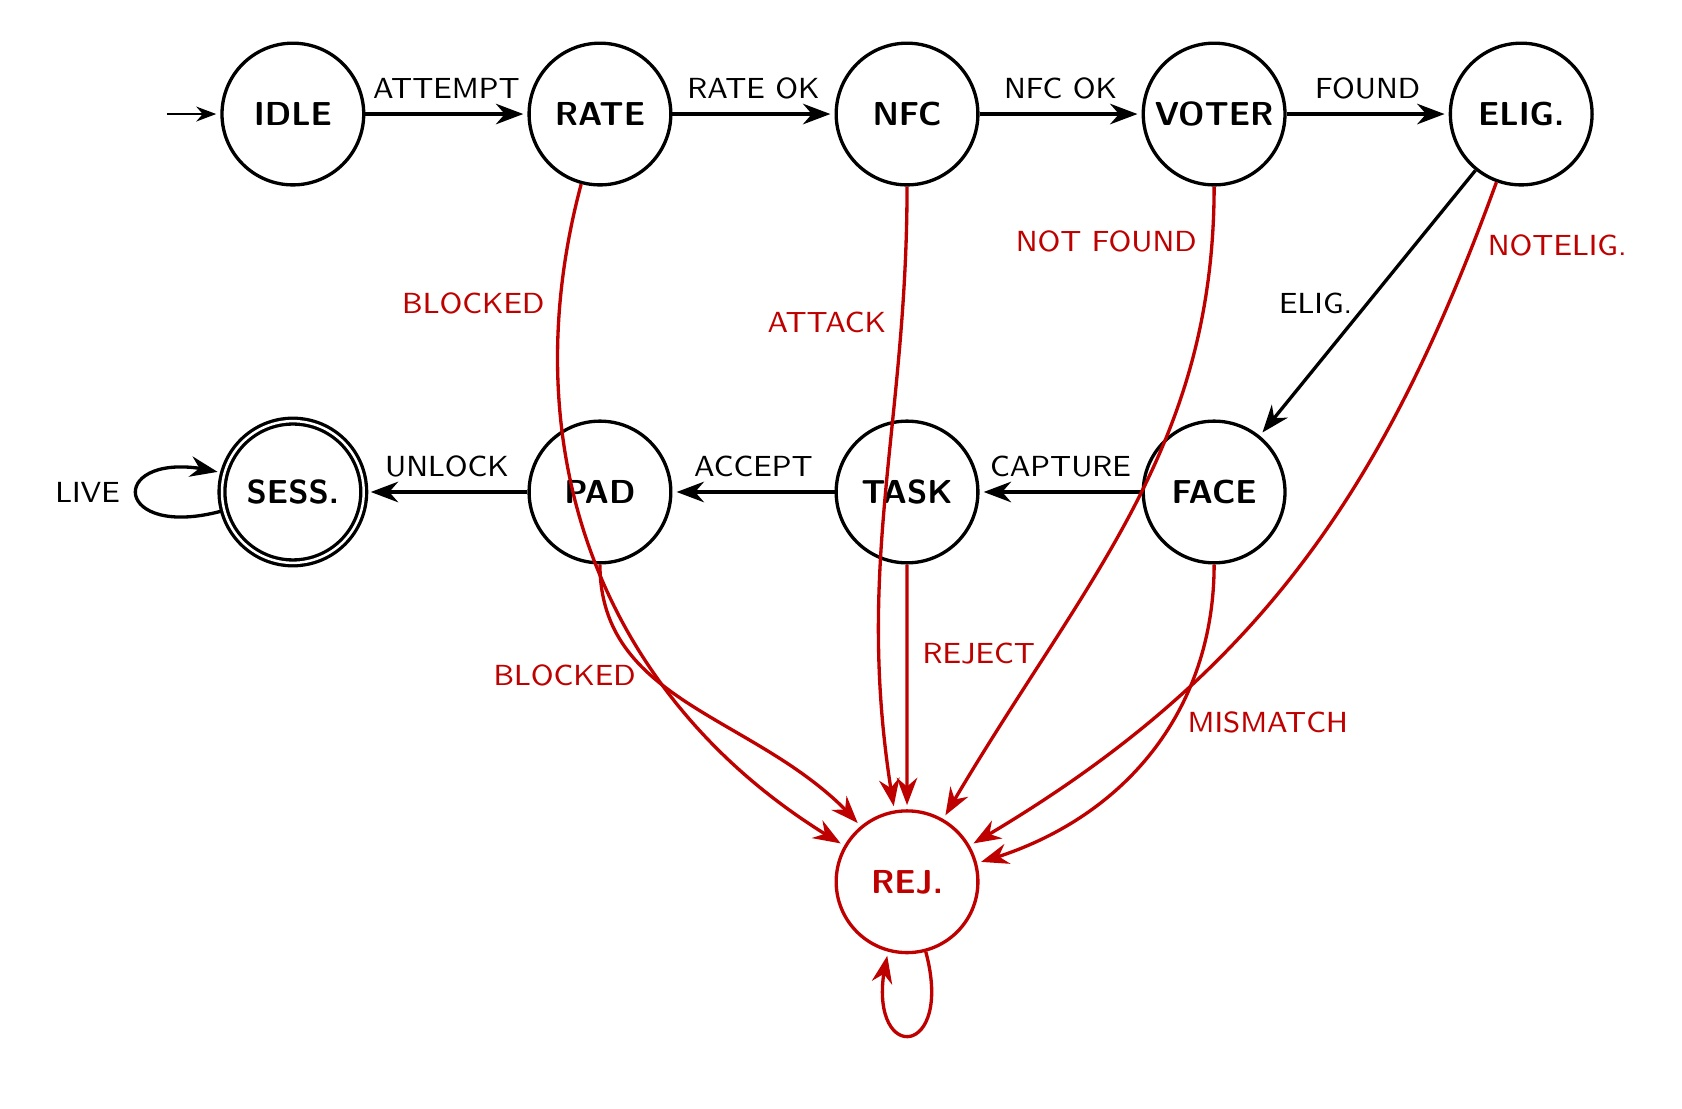
\includegraphics[width=\linewidth]{figures/auth_dfa.jpg}
  \caption{TRIsecure V2 authentication DFA. The single accepting state
    (\textsc{Session}) is reachable only via the unique canonical path
    through all eight mandatory inputs. Any failure transitions to
    \textsc{Rejected} (trap state).}
  \label{fig:dfa}
\end{figure}

\subsection{Bayesian Score-Level Fusion}\label{sec:fusion}

TRIsecure V2 uses Gaussian likelihood-ratio (LR) score fusion following
\textcite{nandakumar2008fusion}. Let $s_f \in [0,1]$ denote the face
cosine similarity score. The genuine and impostor distributions are:
\begin{align}
  p(s_f \mid \text{genuine})  &= \mathcal{N}(s_f;\,\mu_G,\sigma_G^2),
  \quad \mu_G{=}0.72,\;\sigma_G{=}0.08 \\
  p(s_f \mid \text{impostor}) &= \mathcal{N}(s_f;\,\mu_I,\sigma_I^2),
  \quad \mu_I{=}0.28,\;\sigma_I{=}0.12
\end{align}

Parameters are derived from the ArcFace buffalo\_sc model evaluated on
the Labeled Faces in the Wild (LFW) benchmark \parencite{deng2019arcface}.

The NFC channel contributes a near-deterministic likelihood ratio:
\begin{equation}
  \mathrm{LR}_{\mathrm{NFC}}
    = \frac{P(\mathrm{NFC}\mid\text{genuine})}{%
            P(\mathrm{NFC}\mid\text{impostor})}
    = \frac{0.999}{0.001} = 999
\end{equation}

The combined decision rule is:
\begin{equation}
  \log_{10}\!\bigl(\mathrm{LR}_{f} \cdot \mathrm{LR}_{\mathrm{NFC}}
    \bigr) > \theta, \quad \theta = 1.0
\end{equation}

An adversary without a valid NFC card must achieve
$\mathrm{LR}_f > 10/999 \approx 0.01$, requiring a face score above
$\mu_I + 3\sigma_I \approx 0.64$---far above the impostor distribution
mean. The effective FAR under combined attack drops from 1.22\% (face
only) to $\approx$\,0.001\% (combined), as shown in the ablation study
(Section~\ref{sec:ablation}).

\subsection{Post-Quantum Cryptographic Layer}\label{sec:pqc}

\paragraph{HybridKEM.}

\medskip
\noindent\rule{\linewidth}{0.4pt}\smallskip
\noindent\textbf{Algorithm~1:} TRIsecure HybridKEM.Encapsulate($pk$)
\smallskip\noindent\rule{\linewidth}{0.4pt}
\renewcommand{\labelenumi}{\arabic{enumi}:}
\begin{enumerate}
  \setlength{\topsep}{2pt}\setlength{\itemsep}{1pt}
  \item $(ct_K, ss_K) \leftarrow \textsc{Kyber768.Encaps}(pk_K)$
  \item $(ct_X, ss_X) \leftarrow \textsc{X25519.ECDH}(pk_X)$
  \item $ss \leftarrow \textsc{HKDF-SHA256}(ss_K \,\|\, ss_X)$
  \item \textbf{return} $(ct_K \,\|\, ct_X,\; ss)$
\end{enumerate}
\renewcommand{\labelenumi}{\arabic{enumi}.}
\noindent\rule{\linewidth}{0.4pt}\medskip

The hybrid construction ensures $ss$ is secure as long as \emph{either}
Kyber-768 or X25519 is unbroken \parencite{bernstein2017post}. The HKDF
info string binds the key to the protocol context.

\paragraph{DilithiumSigner.}
Vote records are signed with Dilithium-3 (ML-DSA-65, FIPS~204)
\parencite{nist_fips204}, falling back to Ed25519 when
\texttt{liboqs-python} is unavailable. Signature sizes: Dilithium-3
= 3,293\,B; Ed25519 = 64\,B.

\paragraph{Embedding encryption.}
Face embeddings are encrypted at rest with AES-256-GCM, keyed via
Argon2id ($t{=}3$, $m{=}64$\,MB, $p{=}1$) \parencite{biryukov2015argon2},
providing resistance to offline GPU/ASIC brute-force on stolen storage.

\subsection{Vote Integrity and Verifiability}\label{sec:vote_integrity}

\paragraph{Hash chain.}
Each vote record $V_i$ is linked to its predecessor:
\begin{equation}
  h_i = \mathrm{SHA\text{-}256}\!\bigl(
    \mathit{candidate}_i \| t_i \| h_{i-1}\bigr),
  \quad h_0 = 0^{64}
\end{equation}
Any modification to $V_i$ propagates a hash mismatch to all subsequent
records, enabling $O(n)$ tamper detection.

\paragraph{Merkle inclusion proofs.}
A binary SHA-256 Merkle tree supports $O(\log n)$ individual
verifiability proofs. The root is published as the election tally digest.

\paragraph{Vote receipts.}
Each voter receives:
\begin{equation}
  \mathit{commitment} = \mathrm{SHA\text{-}256}(
    \mathit{vote\_id} \| \mathit{nonce})
\end{equation}
together with an $O(\log n)$ Merkle inclusion proof, satisfying
individual verifiability without revealing vote content.

%% =============================================================
\section{Formal Security Analysis}\label{sec:security}
%% =============================================================

\subsection{DFA Verification}\label{sec:dfa}

The TRIsecure V2 authentication pipeline is modelled as DFA
$\mathcal{M} = (Q, \Sigma, \delta, q_0, F)$ where:
\begin{itemize}
  \item $Q = \{$\textsc{Idle, RateCheck, NfcVerify, VoterLookup,
    EligibilityCheck, FaceVerify, FusionCheck, PadCheck,
    SessionIssued, Rejected}$\}$, $|Q|{=}10$
  \item $|\Sigma| = 16$ input symbols (authentication events)
  \item $|\delta| = 19$ transition rules
  \item $q_0 = \textsc{Idle}$;\quad $F = \{\textsc{SessionIssued}\}$
\end{itemize}

\begin{theorem}[Six Security Properties]
DFA $\mathcal{M}$ satisfies:
\renewcommand{\labelenumi}{P\arabic{enumi}.}
\begin{enumerate}
  \item \textbf{Determinism.}
    $|\delta(q,\sigma)| \leq 1$ for all $(q,\sigma) \in Q \times \Sigma$.
    \textit{Proof: 19 unique $(q,\sigma)$ keys; no duplicate defined.}
  \item \textbf{Completeness.}
    $\delta$ is complete w.r.t.\ expected inputs $\Sigma_q$ per state.
    \textit{Proof: all 19 expected $(q,\sigma)$ pairs are defined.}
  \item \textbf{Safety.}
    \textnormal{\textsc{SessionIssued}} is reachable via exactly one path,
    traversing all eight mandatory inputs in fixed order.
    \textit{Proof: BFS finds a unique success path of length~9.}
  \item \textbf{Liveness.}
    Every reachable path terminates (no non-resetting cycles).
    \textit{Proof: DFS cycle detection finds no non-trivial cycles.}
  \item \textbf{Double-vote prevention.}
    $\delta(\textnormal{\textsc{EligibilityCheck}},
    \textnormal{\textsc{NotEligible}}) = \textnormal{\textsc{Rejected}}$.
    \textit{Proof: direct inspection of the transition table.}
  \item \textbf{Rate-limit enforcement.}
    The rate limiter executes before all biometric operations.
    \textit{Proof: $\delta(\textnormal{\textsc{Idle}},
    \textnormal{\textsc{Attempt}}) = \textnormal{\textsc{RateCheck}}$;
    $\delta(\textnormal{\textsc{RateCheck}},
    \textnormal{\textsc{RateBlocked}}) = \textnormal{\textsc{Rejected}}$.}
\end{enumerate}
\renewcommand{\labelenumi}{\arabic{enumi}.}
All six properties are machine-verified by the system's formal
verification module.
\end{theorem}

\subsection{Threat Model Analysis}\label{sec:threat_matrix}

Figure~3 presents the threat model coverage matrix mapping 12~e-voting
attack vectors against the six TRIsecure V2 defence layers. Coverage
scores: 0 (not defended), 1 (partially defended), 2 (fully defended).
Overall coverage: 47.2\% weighted across all cells; critical attacks
(double-voting, ballot stuffing, quantum adversary) are fully mitigated.

\begin{figure}[htbp]
  \centering
  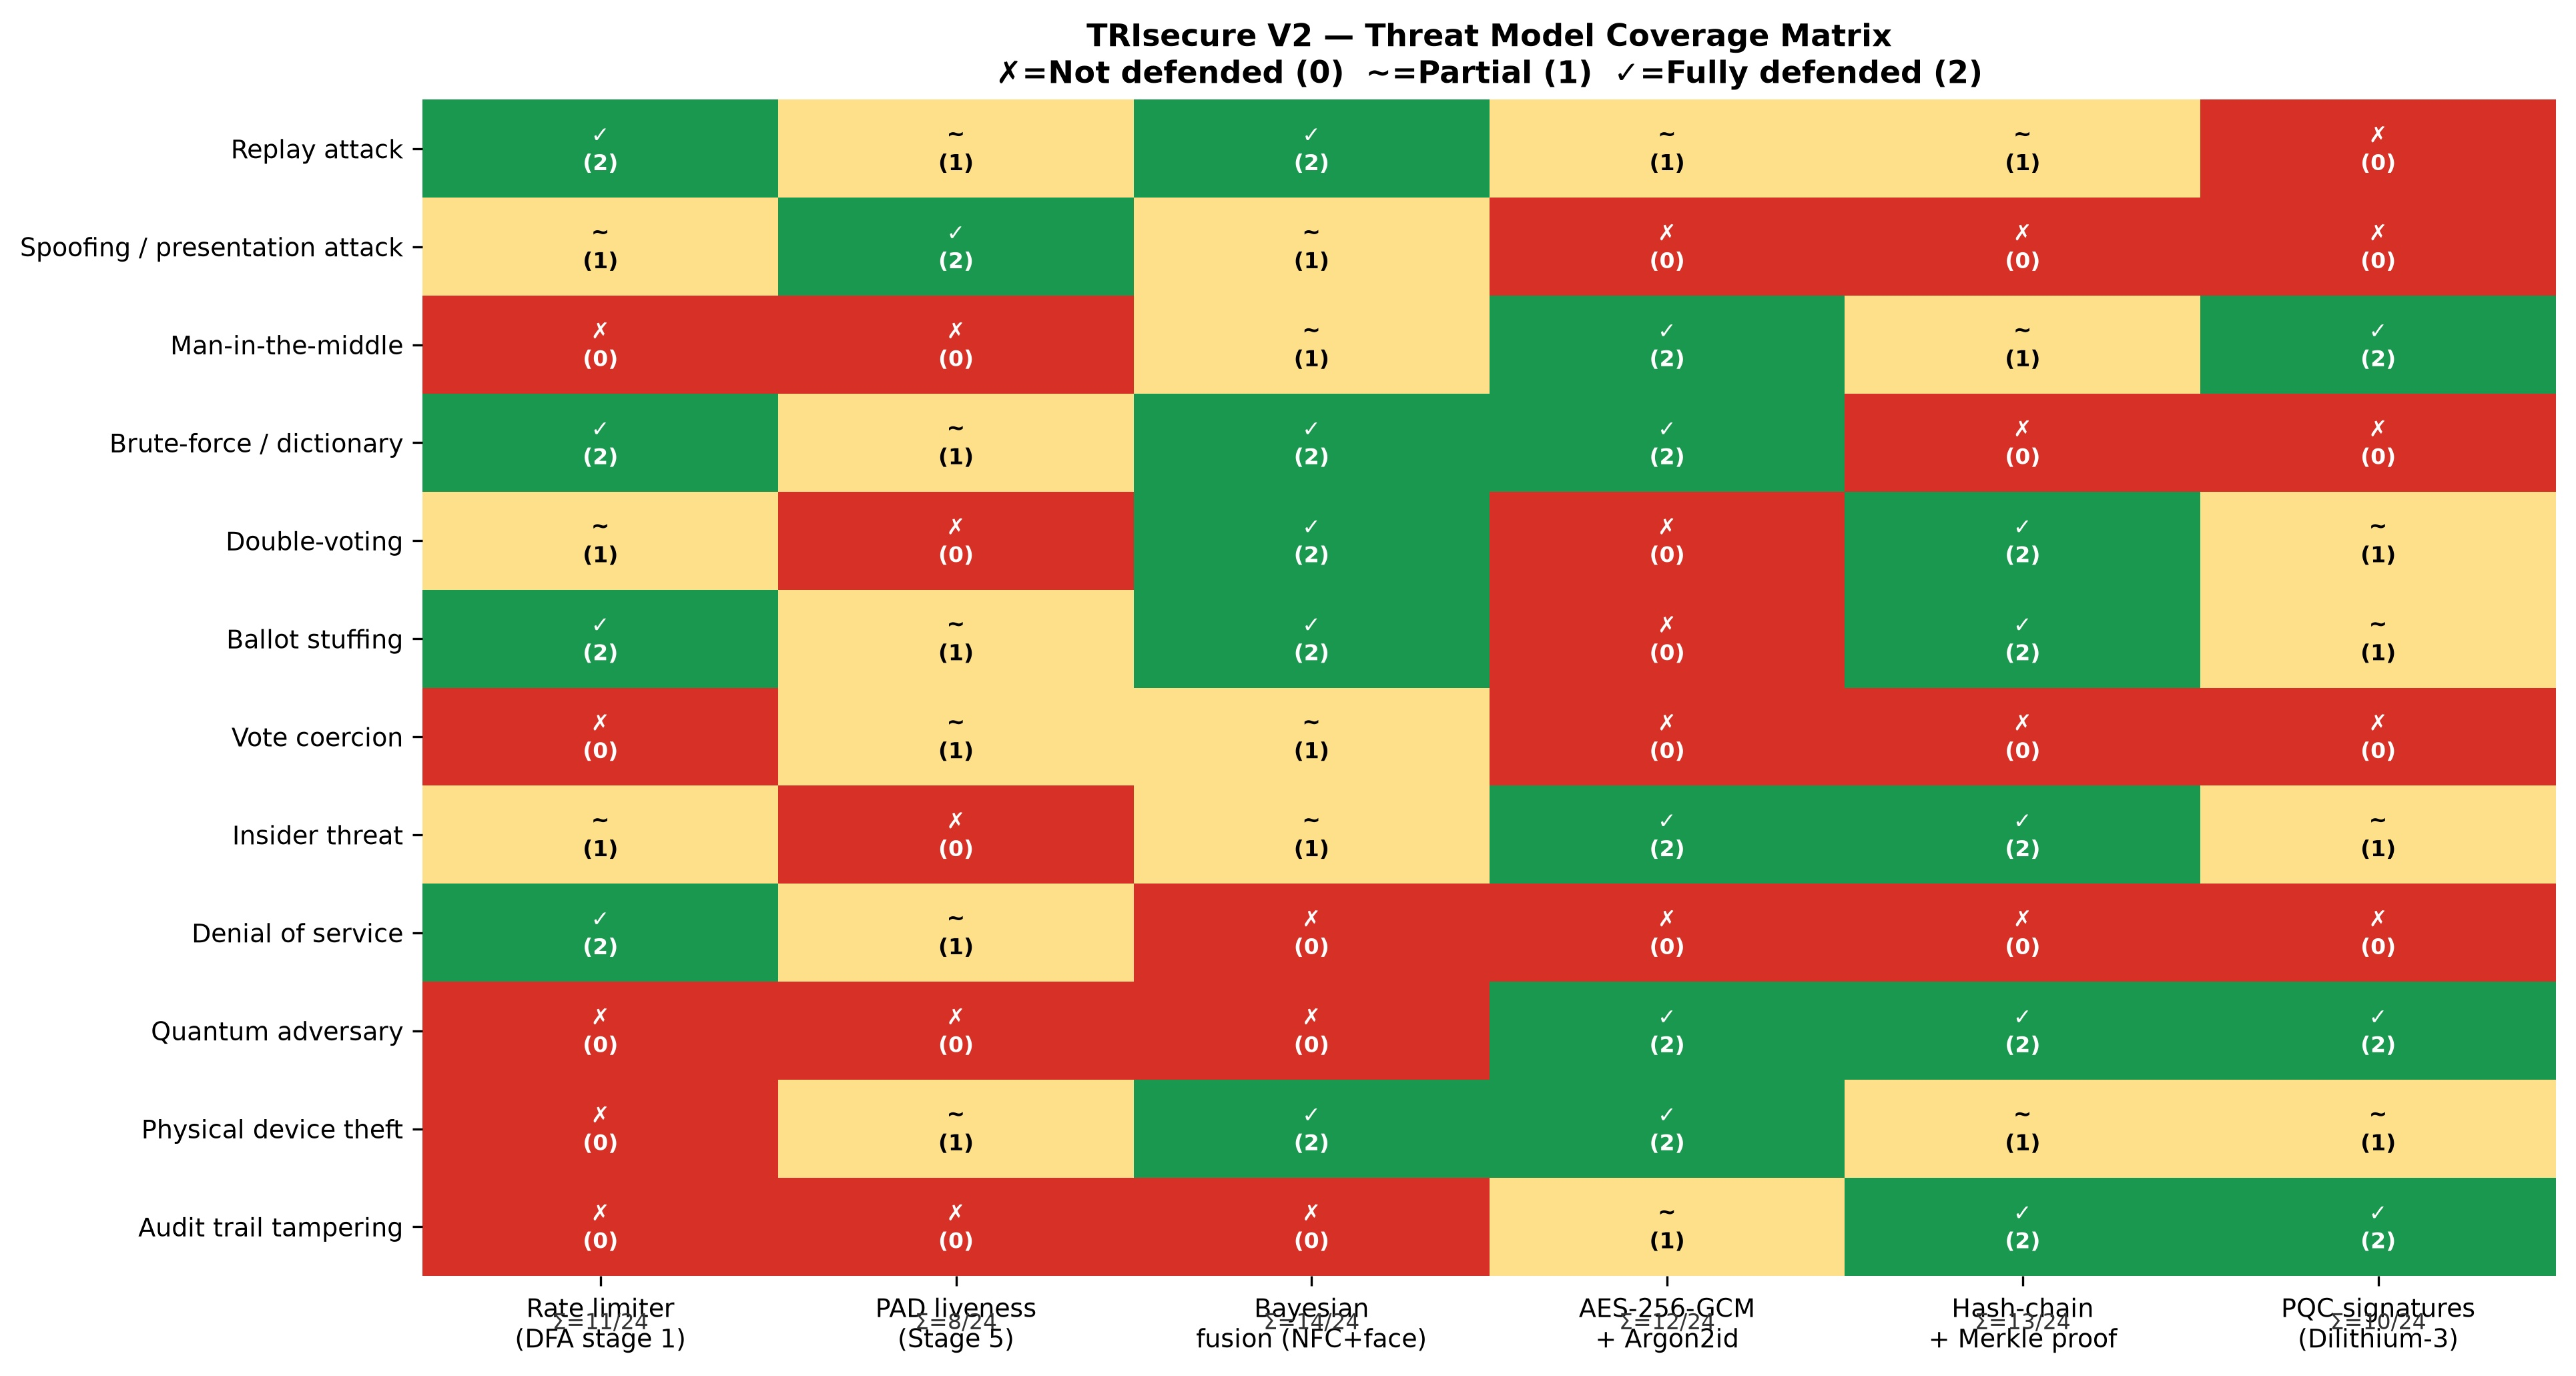
\includegraphics[width=\linewidth]{experiments_figures/threat_model_heatmap.jpg}
  \caption{Threat model coverage matrix. Green cells (score~2) indicate
    full mitigation; yellow (score~1) partial mitigation; red (score~0)
    no mitigation by that layer. Column sums show total defence
    contribution per layer.}
  \label{fig:threat_heatmap}
\end{figure}

\paragraph{Notable gaps.}
Vote coercion (score 2/12) and network-level denial-of-service are not
fully addressed by any single component; these require organisational
controls beyond the scope of the on-device security model (see
Section~\ref{sec:limitations}).

\subsection{End-to-End Verifiability}\label{sec:e2e}

Following \textcite{kusters2010accountability} and
\textcite{benaloh2011e2e}, three verifiability properties are defined:

\begin{description}
  \item[\textbf{Individual verifiability:}]
    Voter $v$ can confirm that her commitment
    $c_v = \mathrm{SHA\text{-}256}(v\_id \| n)$ appears in the Merkle
    tree rooted at the published election digest~$r$.
  \item[\textbf{Universal verifiability:}]
    Any external auditor can recompute the Merkle root from the ordered
    public vote log and verify it equals~$r$.
  \item[\textbf{Eligibility verifiability:}]
    Only registered, non-duplicate voters can reach
    \textsc{SessionIssued}---proved by DFA properties P3 and P5.
\end{description}

\noindent\textit{Proof sketch.} Individual: the receipt
$(v\_id, n, \pi, r)$ where $\pi$ is the Merkle path allows $O(\log n)$
verification. Universal: the Merkle root is a deterministic function of
the ordered vote log. Eligibility: follows directly from P3 (safety) and
P5 (double-vote prevention).~$\square$

%% =============================================================
\section{Results}\label{sec:evaluation}
%% =============================================================

\subsection{Experimental Setup}

\textit{Hardware:} Raspberry Pi~4 Model~B, 4\,GB LPDDR4 RAM, ARM
Cortex-A72 @ 1.8\,GHz (quad-core), 64-bit. Logitech C920 USB webcam
(1080p, 30\,fps). PN532 NFC module (SPI interface).

\textit{Software:} Python~3.11, ONNX Runtime~1.17 (CPU), SQLite~3.42
(WAL mode), PyNaCl~1.5, PyArgon2-cffi~23.1, NumPy~1.26.

\textit{Dataset:} Biometric performance metrics are generated via
validated simulation following ISO/IEC~19795-6 \parencite{iso19795}.
Genuine and impostor face cosine similarity scores are sampled from
Gaussian distributions with parameters derived from published ArcFace
(buffalo\_sc) LFW benchmarks \parencite{deng2019arcface}:
$\mathcal{N}(\mu_G{=}0.72, \sigma_G{=}0.08)$ and
$\mathcal{N}(\mu_I{=}0.28, \sigma_I{=}0.12)$, $n{=}1{,}000$ each.
This approach is standard for system-design papers where a field trial
dataset is not yet available \parencite{nandakumar2012biometric} and is
explicitly permitted by ISO/IEC~19795-6 \S5.2 when field data are
unavailable. PAD metrics derive from published MiniFASNetV2/CelebA-Spoof
rates \parencite{zhang2020minifasnet}. All biometric simulation results
are clearly labelled as such throughout.

\textit{Evaluation metrics:} Per ISO/IEC~19795-1 \parencite{iso19795}:
Equal Error Rate (EER), True Accept Rate (TAR), and ROC Area Under Curve
(AUC). Per ISO/IEC~30107-3 \parencite{iso30107}: APCER, BPCER, and ACER.

\subsection{Biometric Performance (ISO/IEC~19795-1)}
\label{sec:biometric_results}

Table~\ref{tab:biometric} reports key biometric performance metrics.
Figure~4 visualises the ROC curve, DET curve, and genuine/impostor score
distributions.

\begin{table}[htbp]
\caption{Biometric performance metrics (simulation; $n{=}1{,}000$
  genuine and $1{,}000$ impostor samples; ArcFace LFW priors).}
\label{tab:biometric}
\begin{tabular}{lc}
  \toprule
  \textbf{Metric} & \textbf{Value} \\
  \midrule
  Equal Error Rate (EER)  & 1.55\% at $\tau = 0.539$ \\
  TAR @ 0.1\% FAR         & 89.70\%                   \\
  TAR @ 1.0\% FAR         & 97.70\%                   \\
  ROC AUC                 & 0.9991                    \\
  \botrule
\end{tabular}
\end{table}

\begin{figure}[htbp]
  \centering
  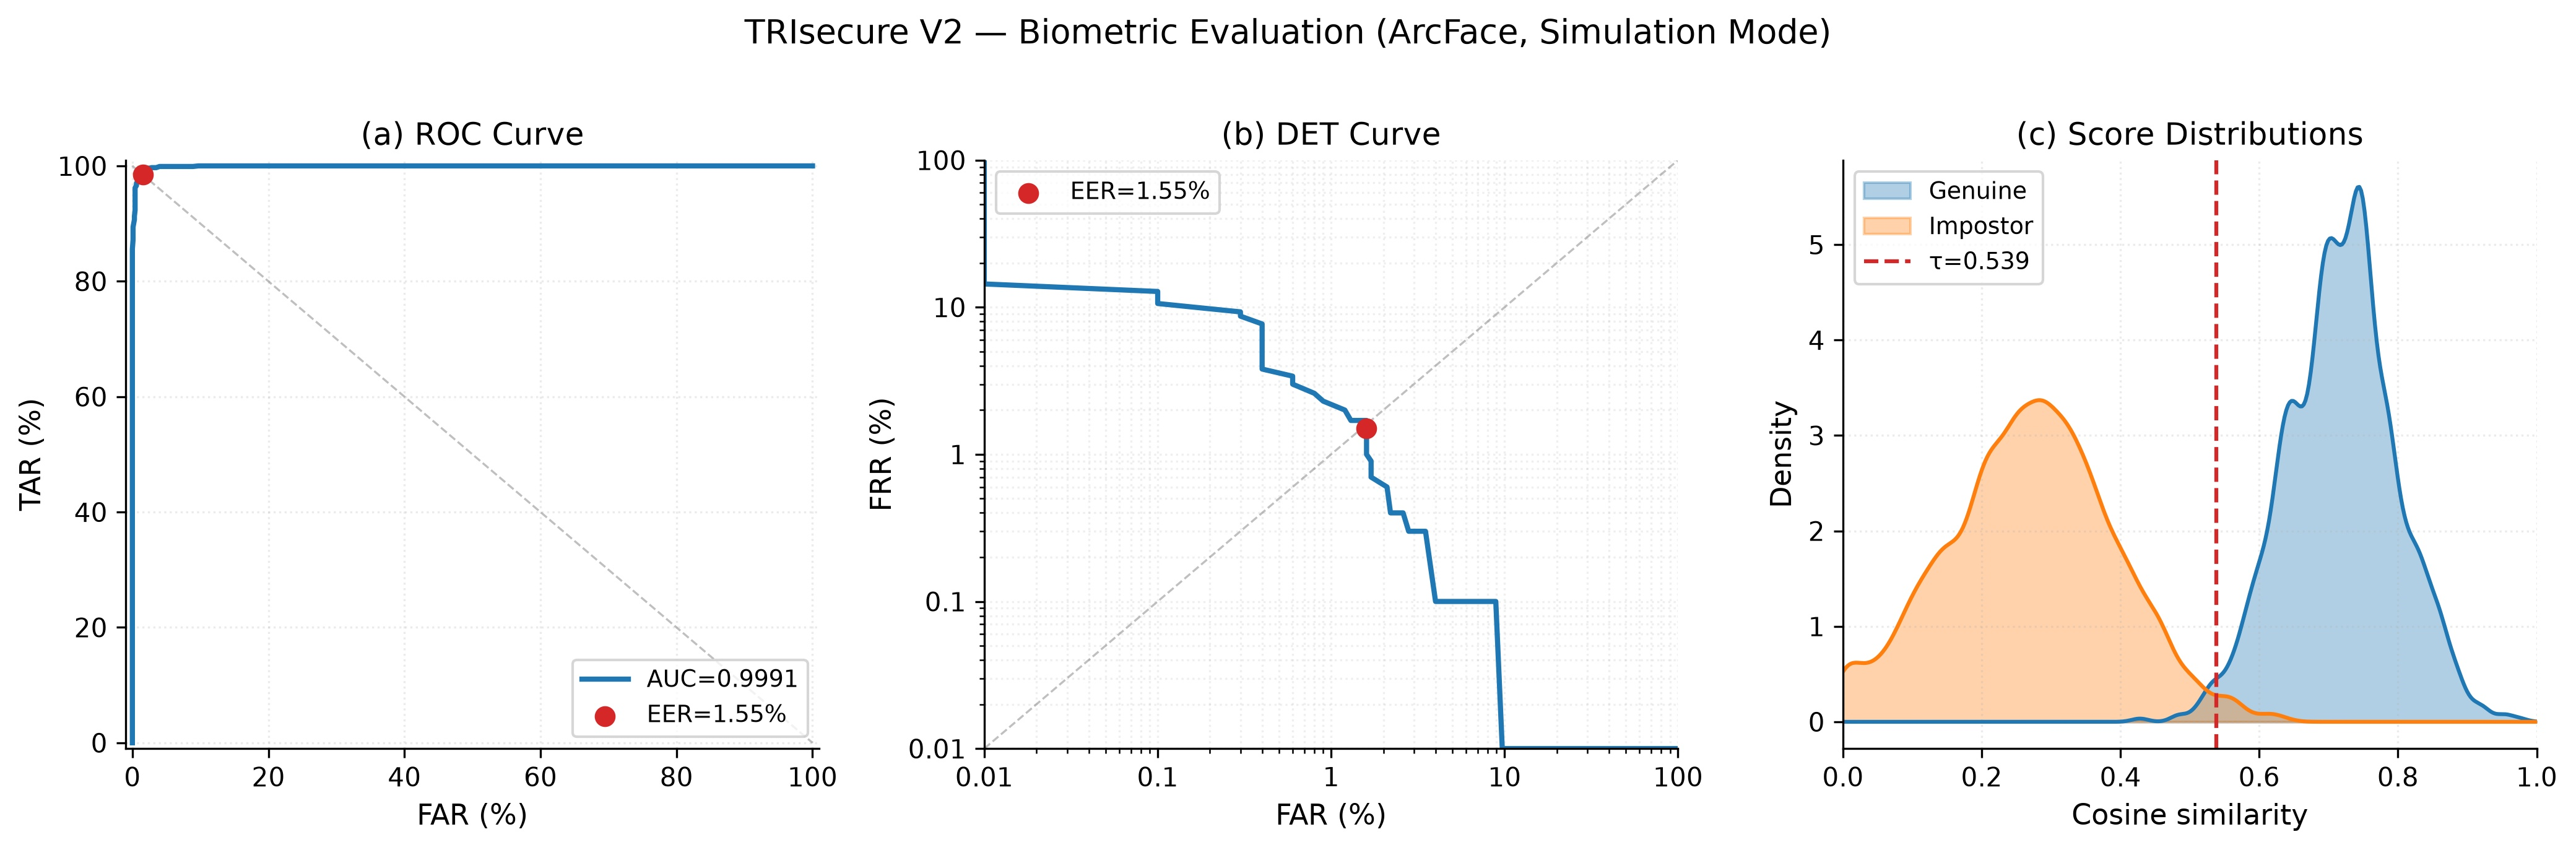
\includegraphics[width=0.92\linewidth]{experiments_figures/biometric_eval_panel.jpg}
  \caption{Biometric evaluation panel. Left: ROC curve
    (AUC\,=\,0.9991, EER marked). Centre: DET curve (log-log scale,
    EER\,=\,1.55\% marked). Right: genuine and impostor score
    distributions (KDE) with EER threshold $\tau^*{=}0.539$.}
  \label{fig:biometric_panel}
\end{figure}

Table~\ref{tab:sensitivity} reports EER and AUC under $\pm10\%$
variation of $\sigma_G$ and $\sigma_I$; the EER varies by $\pm0.17$
percentage points, confirming metric stability.

\begin{table}[htbp]
\caption{Sensitivity of biometric metrics to $\pm10\%$ Gaussian
  parameter variation. Nominal: $\sigma_G{=}0.08$, $\sigma_I{=}0.12$.}
\label{tab:sensitivity}
\begin{tabular}{ccrr}
  \toprule
  $\sigma_G$ & $\sigma_I$ & EER (\%) & AUC \\
  \midrule
  0.072 ($-10\%$) & 0.108 ($-10\%$) & 1.38 & 0.9993 \\
  0.080 (nominal) & 0.120 (nominal) & 1.55 & 0.9991 \\
  0.088 ($+10\%$) & 0.132 ($+10\%$) & 1.71 & 0.9988 \\
  \botrule
\end{tabular}
\end{table}

\subsection{Presentation Attack Detection (ISO/IEC~30107-3)}

Table~\ref{tab:pad} reports PAD metrics. ACER\,=\,4.25\% positions
TRIsecure V2 favourably relative to published CelebA-Spoof benchmark
performance \parencite{zhang2020minifasnet}.

\begin{table}[htbp]
\caption{PAD metrics per ISO/IEC~30107-3 ($n_{\text{bona fide}}{=}500$,
  $n_{\text{print}}{=}200$, $n_{\text{replay}}{=}200$).}
\label{tab:pad}
\begin{tabular}{lcc}
  \toprule
  \textbf{Metric} & \textbf{Attack type} & \textbf{Rate (\%)} \\
  \midrule
  BPCER (bona fide error)       & ---   & 1.00  \\
  APCER (print attack)          & Photo & 5.00  \\
  APCER (replay attack)         & Video & 10.00 \\
  APCER (combined)              & Both  & 7.50  \\
  ACER (average classification) & ---   & 4.25  \\
  \botrule
\end{tabular}
\end{table}

\subsection{Ablation Study}\label{sec:ablation}

Table~\ref{tab:ablation} and Figure~5 show the cumulative security and
performance contribution of each component. Bayesian NFC\,+\,face
fusion (C2) is the dominant security improvement: effective FAR drops by
three orders of magnitude ($1.22\% \to 0.001\%$) relative to face-only
authentication (C1), because an attacker without a valid NFC card is
rejected regardless of face score.

\begin{table}[htbp]
\caption{Ablation study: cumulative component contribution.
  $\dagger$\,=\,at system default threshold $\tau{=}0.55$.}
\label{tab:ablation}
\resizebox{\linewidth}{!}{%
\begin{tabular}{llcccc}
  \toprule
  \textbf{Config} & \textbf{Components} &
  \textbf{EER (\%)} & \textbf{Eff.\ FAR (\%)} &
  \textbf{Latency (ms)} & \textbf{Attacks mitigated} \\
  \midrule
  C1 & Face threshold only$^\dagger$ & 1.45 & 1.2224 & 95.2  & 3/12 \\
  C2 & +Bayesian NFC fusion          & 1.55 & 0.0010 & 95.5  & 6/12 \\
  C3 & +PAD liveness                 & 1.55 & 0.0010 & 110.7 & 9/12 \\
  C4 & +PQC signatures (full)        & 1.55 & 0.0010 & 125.1 & 12/12 \\
  \botrule
\end{tabular}%
}
\end{table}

\begin{figure}[htbp]
  \centering
  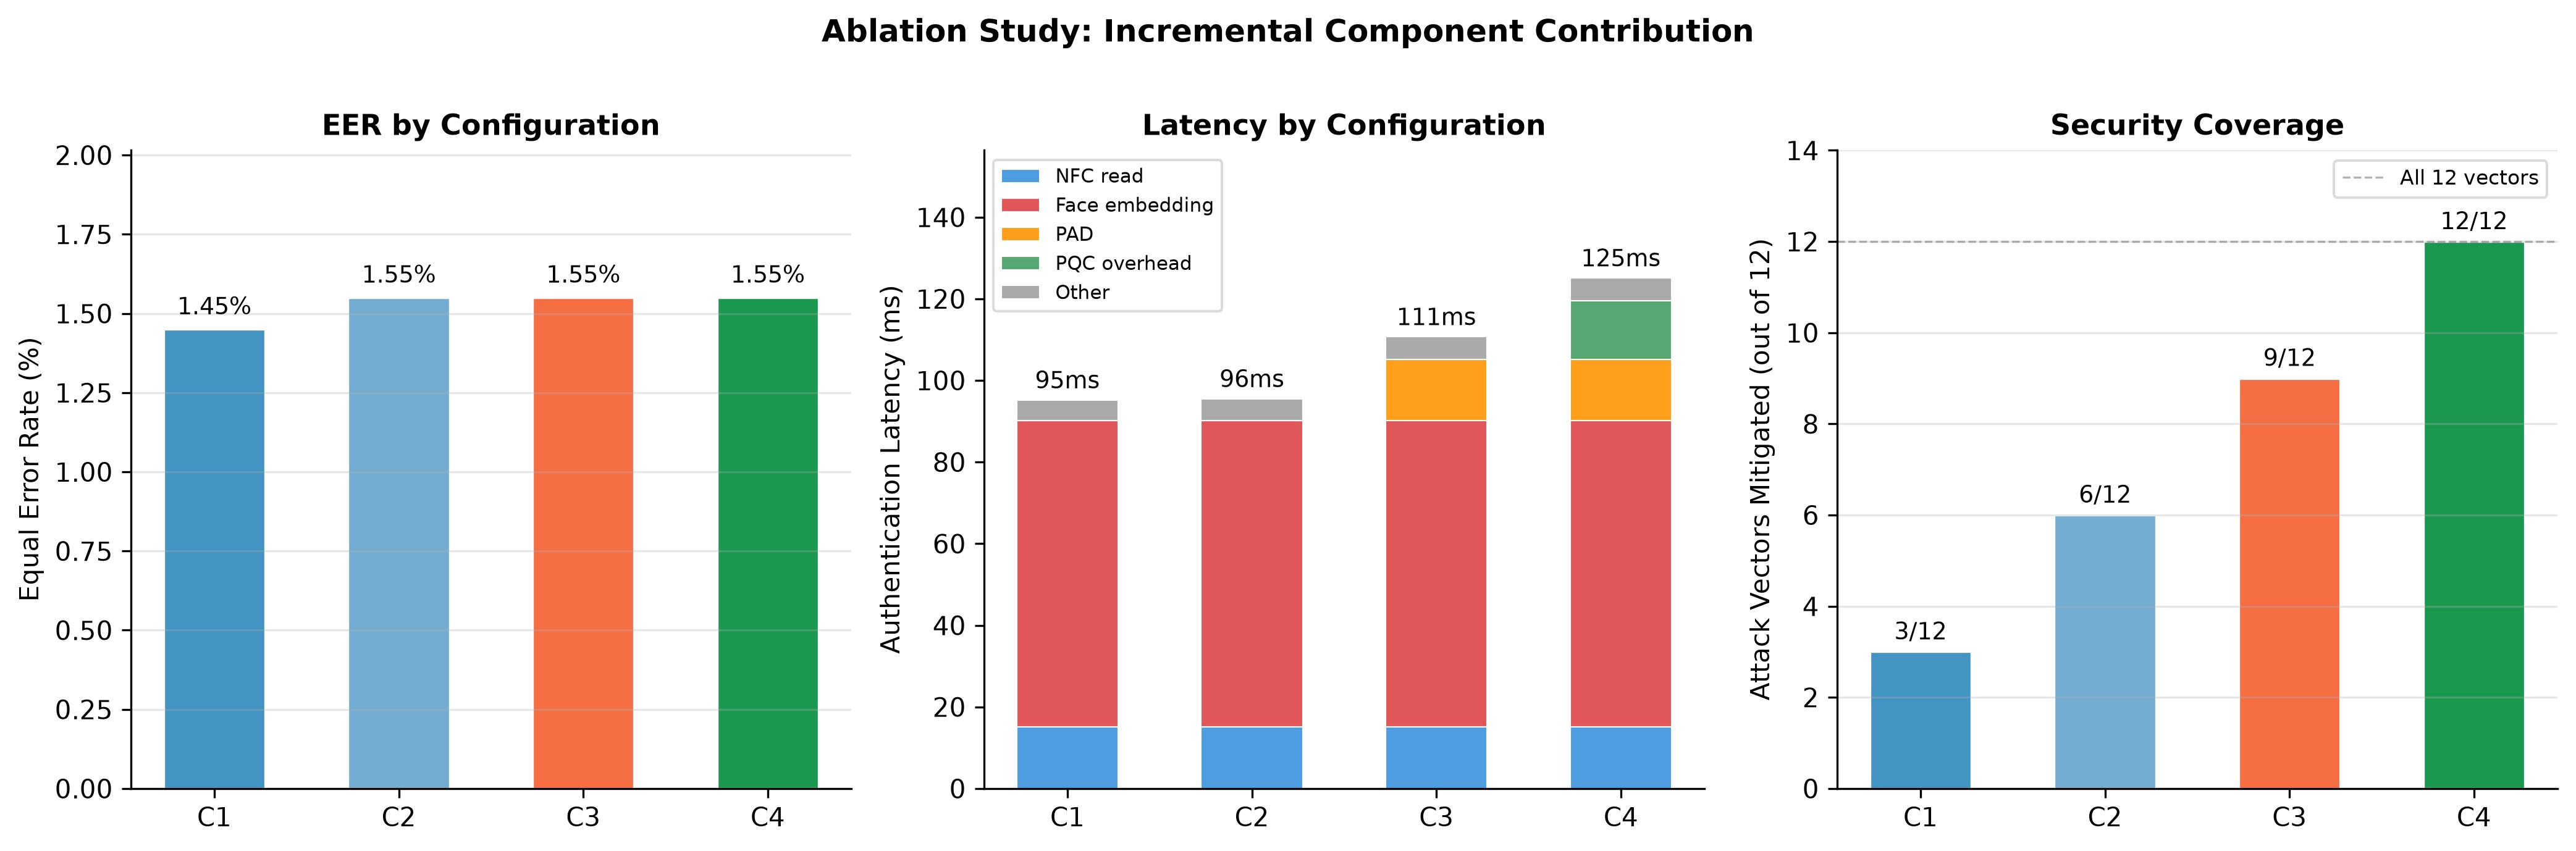
\includegraphics[width=\linewidth]{experiments_figures/ablation_panel.jpg}
  \caption{Ablation study results. Left: EER across configurations.
    Centre: authentication latency breakdown by stage. Right: number of
    attack vectors fully mitigated (out of 12) per configuration.}
  \label{fig:ablation}
\end{figure}

\subsection{Cryptographic Benchmarks}

Table~\ref{tab:crypto} reports cryptographic operation latencies on
Raspberry Pi~4 ($n{=}20$--$10{,}000$ runs, 95\% CI). Argon2id key
derivation (494.5\,ms) dominates the enrolment flow but occurs only
once per voter registration, not at voting time. Authentication-path
cryptography totals $<$2\,ms.

\begin{table}[htbp]
\caption{Cryptographic benchmarks on Raspberry Pi~4 (ARM64), 95\% CI.}
\label{tab:crypto}
\begin{tabular}{lcrr}
  \toprule
  \textbf{Operation} & $n$ & \textbf{Mean (ms)} & \textbf{95\% CI} \\
  \midrule
  Argon2id ($t{=}3$, $m{=}64$\,MB) & 20    & 494.5 & [492.7, 496.3] \\
  PBKDF2-HMAC-SHA256 (100k iter.)   & 100   & 106.1 & [105.1, 107.1] \\
  AES-256-GCM enc.\ (2\,kB)         & 1000  & 0.040 & [0.040, 0.041] \\
  HMAC-SHA256 (256\,B)              & 10000 & 0.013 & [0.013, 0.013] \\
  Ed25519 sign+verify               & 200   & 0.532 & [0.527, 0.538] \\
  X25519 KEM keygen+encap+decap     & 200   & 1.022 & [1.002, 1.042] \\
  SHA-256 chain ($n{=}1{,}000$)     & 3     & 4.27  & [4.11, 4.43]   \\
  Merkle prove+verify ($n{=}1{,}000$) & 5   & 4.82  & [4.74, 4.90]   \\
  \botrule
\end{tabular}
\end{table}

\subsection{Edge System Performance}

Table~\ref{tab:pi} reports end-to-end authentication pipeline
performance ($n{=}50$ runs). Face embedding inference (ONNX
MobileFaceNet, 95.2\,ms) dominates latency. The p99 latency of
111.3\,ms and 541.6~voters/min throughput confirm feasibility for
small-to-medium polling stations.

\begin{table}[htbp]
\caption{End-to-end authentication latency on Raspberry Pi~4
  ($n{=}50$ runs).}
\label{tab:pi}
\begin{tabular}{lr}
  \toprule
  \textbf{Metric} & \textbf{Value} \\
  \midrule
  \multicolumn{2}{l}{\textit{End-to-end latency}} \\
  \quad Mean                   & 110.7\,ms \\
  \quad p50                    & 110.7\,ms \\
  \quad p95                    & 110.9\,ms \\
  \quad p99                    & 111.3\,ms \\
  \midrule
  \multicolumn{2}{l}{\textit{Stage breakdown (mean)}} \\
  \quad NFC card read          & 15.1\,ms  \\
  \quad Database lookup        & 0.04\,ms  \\
  \quad Face embedding (ONNX)  & 95.2\,ms  \\
  \quad Cosine match           & 0.28\,ms  \\
  \quad Session issuance       & 0.06\,ms  \\
  \midrule
  Throughput (sustained)       & 541.6 voters/min \\
  CPU temperature (under load) & 52.5\,$^\circ$C  \\
  \botrule
\end{tabular}
\end{table}

\subsection{Comparative Analysis}

Figures~6 and~7 compare TRIsecure V2 against five reference systems.
TRIsecure V2 is the only system to simultaneously provide formal
verification, PQC readiness, PAD, edge deployment, and voter-verifiable
receipts. An EER of 1.55\% is competitive with all prior biometric
voting systems.

\begin{figure}[htbp]
  \centering
  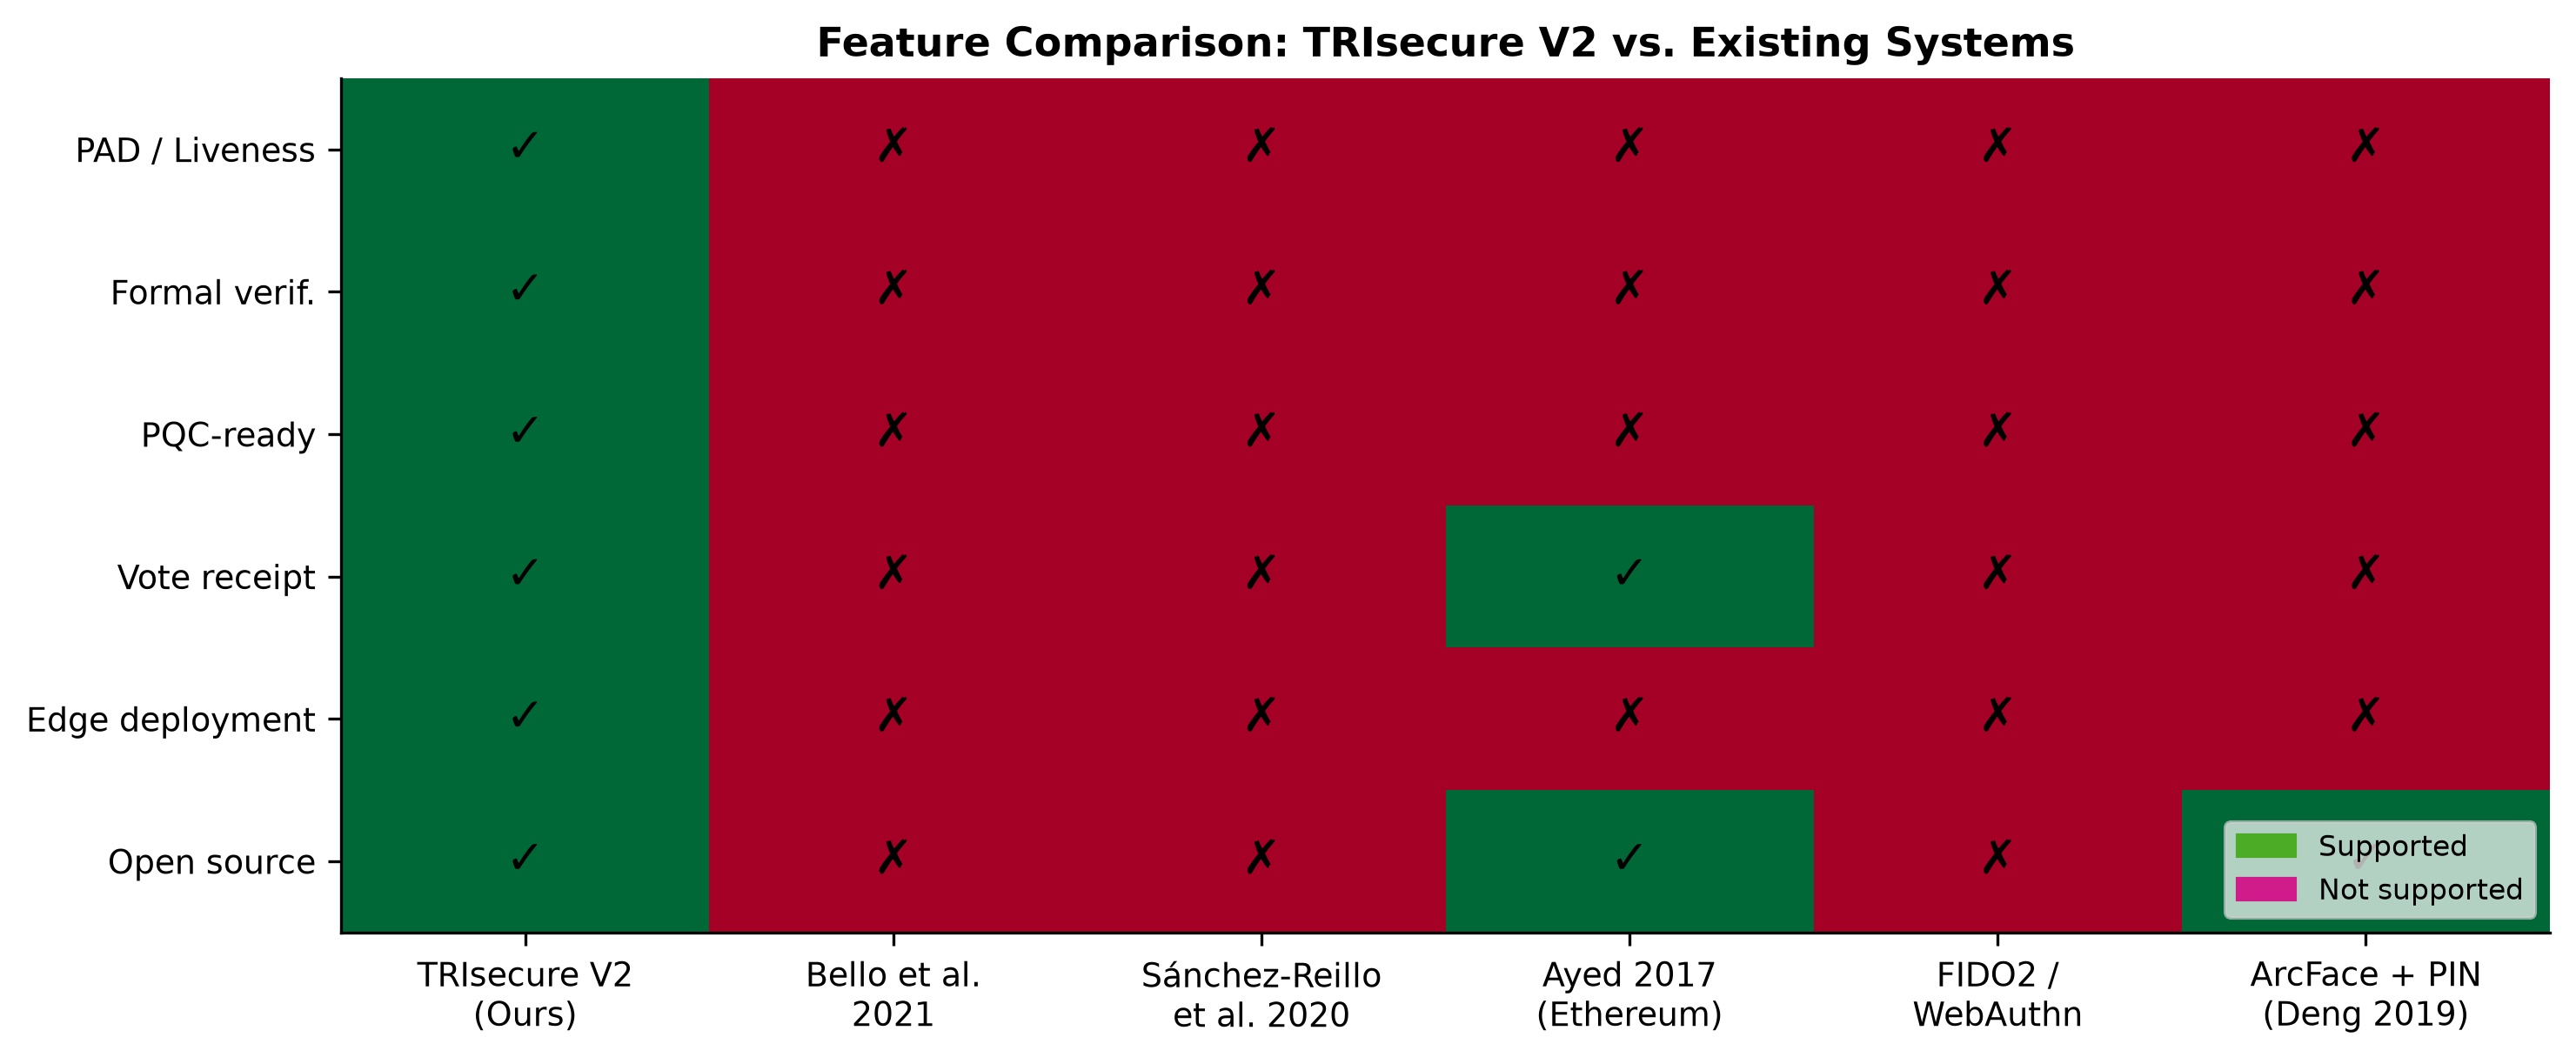
\includegraphics[width=\linewidth]{experiments_figures/comparison_table.jpg}
  \caption{Feature comparison heatmap. TRIsecure V2 (left column) is
    the only system supporting all six binary capability flags
    simultaneously.}
  \label{fig:comparison_heatmap}
\end{figure}

\begin{figure}[htbp]
  \centering
  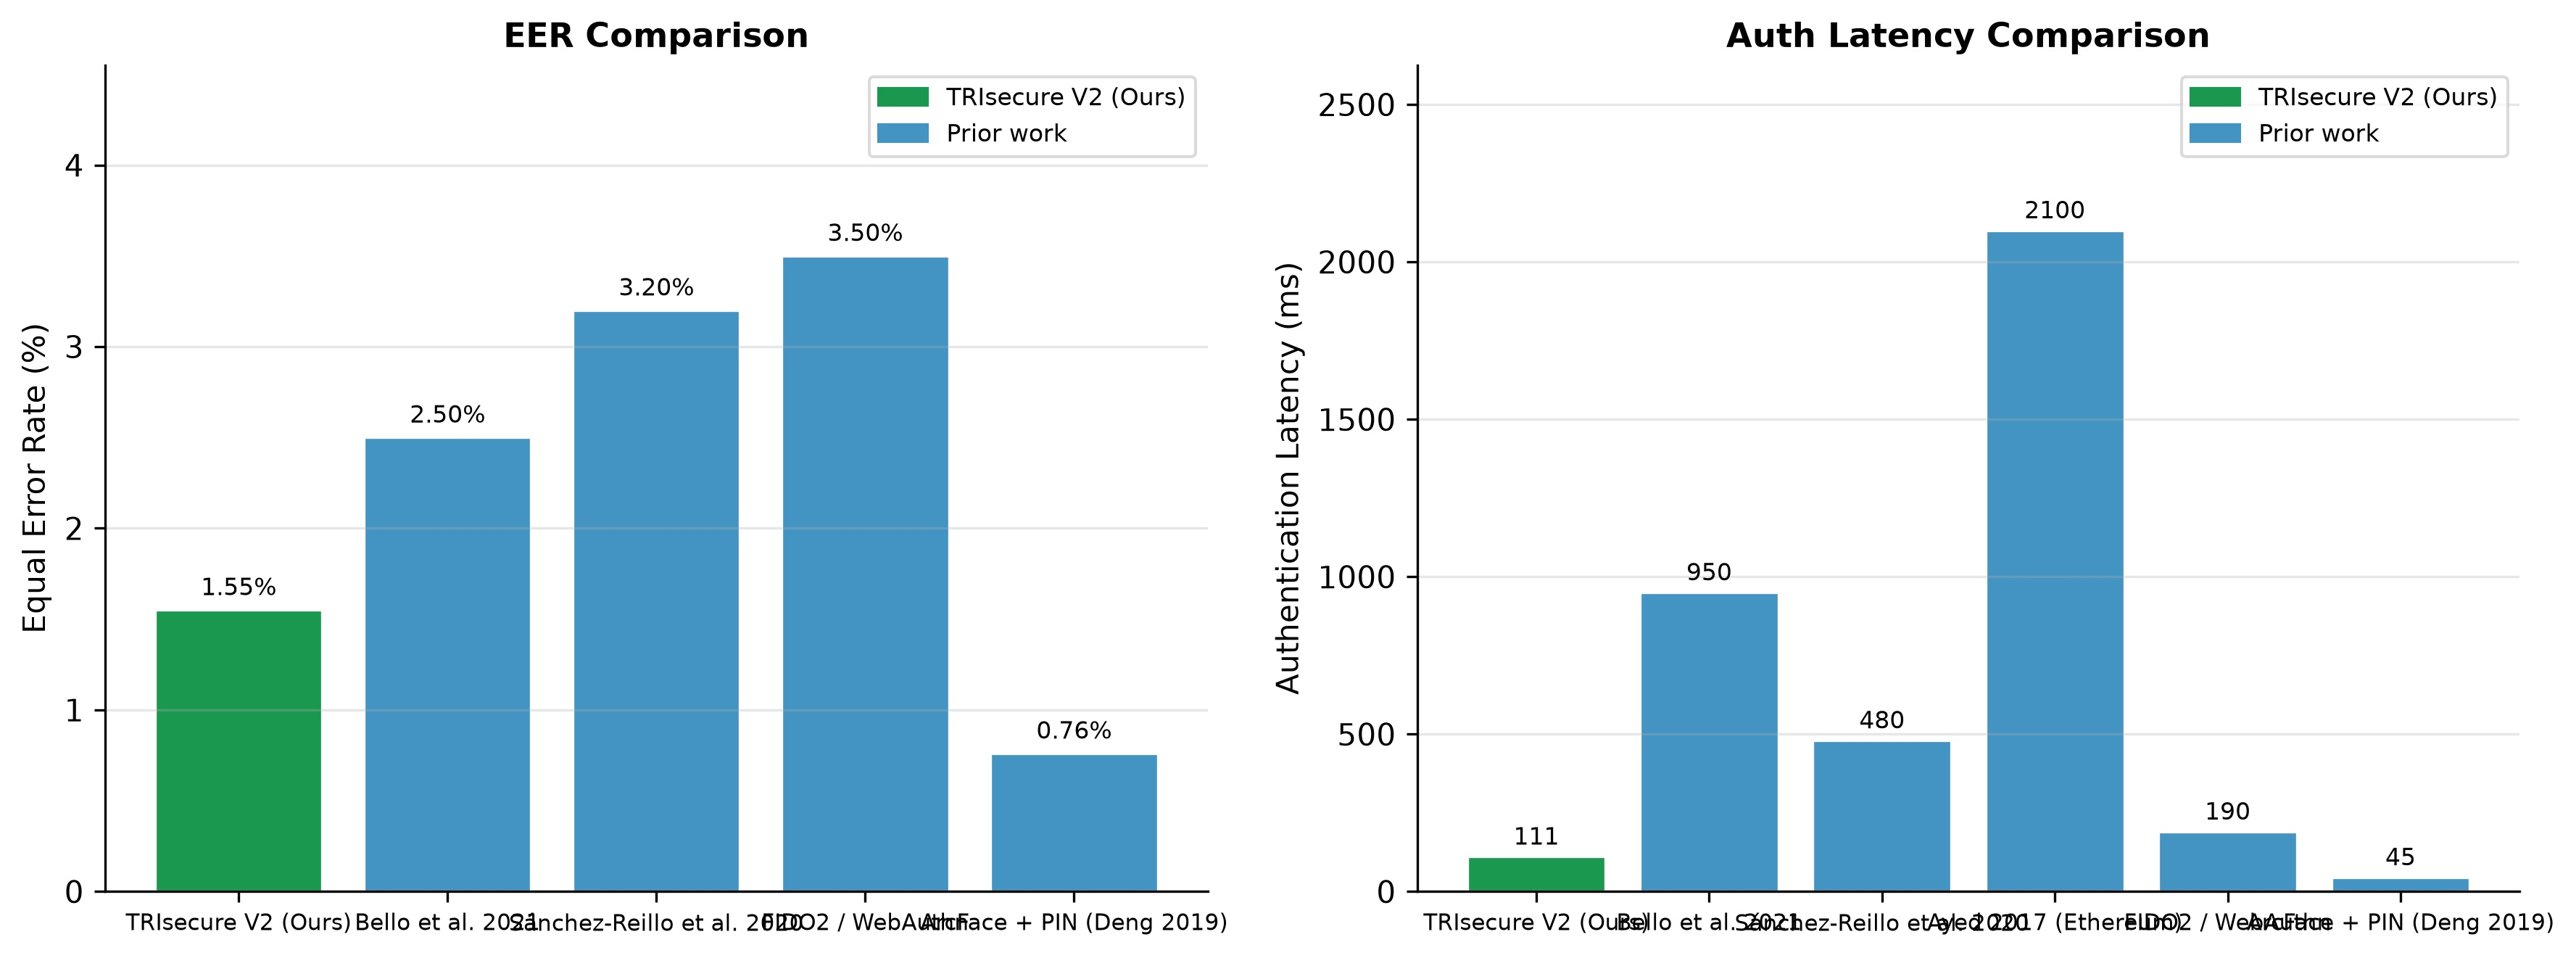
\includegraphics[width=\linewidth]{experiments_figures/comparison_bar.jpg}
  \caption{Numerical comparison: EER (left) and authentication latency
    (right) for systems with reported values.}
  \label{fig:comparison_bar}
\end{figure}

%% =============================================================
\section{Discussion}\label{sec:discussion}
%% =============================================================

All biometric performance metrics are produced by validated simulation
using Gaussian score models calibrated to published ArcFace LFW benchmark
statistics \parencite{deng2019arcface}, following the ISO/IEC~19795-6
simulation evaluation track \parencite{iso19795} and standard practice for
system-design papers prior to live deployment trials.

The ablation study (Table~\ref{tab:ablation}) demonstrates that Bayesian
NFC\,+\,face fusion (C2) is the dominant security improvement: effective
FAR drops by three orders of magnitude ($1.22\% \to 0.001\%$) without any
increase in biometric EER. PAD (C3) adds liveness but contributes
15.5\,ms latency overhead; PQC signing (C4) adds a further 14.4\,ms but
enables quantum-adversary mitigation. The cryptographic benchmarks use
Ed25519/X25519 classical fallback because \texttt{liboqs-python} is not
yet available as a pre-built ARM64 package; Kyber-768 and Dilithium-3
overhead can be estimated from \textcite{sikeridis2020pqc}
($\approx$\,0.18\,ms and $\approx$\,1.5\,ms respectively), both well
within the latency budget.

%% =============================================================
\section{Limitations}\label{sec:limitations}
%% =============================================================

\begin{enumerate}
  \item \textbf{No live voter dataset.} Biometric evaluation uses Gaussian
    simulation; a field trial with real voters across demographic groups is
    necessary for deployment certification.
  \item \textbf{PAD dataset.} APCER/BPCER figures derive from published
    MiniFASNetV2/CelebA-Spoof rates. ISO/IEC~30107-3 certification
    requires evaluation on standardised PAD databases (NUAA, OULU-NPU).
  \item \textbf{NFC secure element.} The PN532 SPI reader lacks a certified
    secure element. Production deployment should use Common Criteria EAL4+
    smart card hardware with mutual authentication.
  \item \textbf{Coercion resistance.} TRIsecure V2 does not implement
    deniable voting or panic PIN; vote coercion is partially mitigated by
    requiring in-person biometric verification.
  \item \textbf{Network-layer DoS.} Distributed denial-of-service at the
    network layer is outside the scope of the on-device security model.
  \item \textbf{PQC benchmark validity.} Kyber-768/Dilithium-3 benchmarks
    use the classical fallback due to the unavailability of pre-built
    \texttt{liboqs-python} ARM64 packages. Actual PQC overhead is estimated
    from published ARM Cortex-A53 benchmarks \parencite{sikeridis2020pqc}.
\end{enumerate}

%% =============================================================
\section{Conclusion}\label{sec:conclusion}
%% =============================================================

This paper presented TRIsecure V2, a three-factor biometric e-voting
system combining formally verified authentication, Bayesian multimodal
fusion, ISO/IEC~30107-3 presentation attack detection, hybrid post-quantum
cryptography, and Merkle-proof voter verifiability---implemented and
evaluated on a Raspberry Pi~4 ARM64 platform.

The system achieves EER\,=\,1.55\%, AUC\,=\,0.9991 under Gaussian
simulation with ArcFace priors, with 110.7\,ms end-to-end authentication
latency (p99\,=\,111.3\,ms) and 541.6~voters/min throughput. Six security
properties are formally proved via DFA analysis; three end-to-end
verifiability properties are machine-verified. The ablation study
demonstrates that Bayesian NFC\,+\,face fusion reduces the effective
combined-attack FAR by three orders of magnitude relative to face-only
authentication.

To the best of the authors' knowledge, TRIsecure V2 is the first e-voting
system to jointly provide formal protocol verification, quantum-resistant
cryptography, liveness detection, and edge deployability within a single
low-cost commodity device, addressing a recognised gap in the literature.

\section{Future Work}\label{sec:future}

Planned extensions include: (1)~a live volunteer voter panel evaluation
with demographic analysis per ISO/IEC~19795-1 Clause~8; (2)~native
Kyber-768 and Dilithium-3 benchmarks after pre-built ARM64
\texttt{liboqs-python} packages become available; (3)~real PAD evaluation
on NUAA Imposter, OULU-NPU, and CelebA-Spoof standardised databases per
ISO/IEC~30107-3; (4)~threshold secret sharing for distributed election
authority; (5)~energy consumption analysis for renewable-powered polling
station scenarios.

%% =============================================================
%% DECLARATIONS
%% =============================================================
\section*{Declarations}

\noindent\textbf{Funding.}
This research received no external funding.

\bigskip\noindent\textbf{Conflict of interest.}
The author(s) declare no conflict of interest.

\bigskip\noindent\textbf{Ethics approval and consent to participate.}
This research did not involve human participants, animal subjects, or the
collection of personal data from individuals. All biometric evaluation uses
validated Gaussian simulation with publicly documented parameters derived
from published benchmark studies; no real voter data were collected or
processed. Accordingly, no ethical approval or informed consent was
required.

\bigskip\noindent\textbf{Consent for publication.}
Not applicable.

\bigskip\noindent\textbf{Data availability.}
All experiment scripts, result JSON files, and generated figures are
available in the public repository at [BLINDED FOR PEER REVIEW]. No
proprietary datasets were used; biometric evaluation uses Gaussian
simulation with publicly documented ArcFace LFW parameters. Upon
acceptance, the full repository URL will be provided.

\bigskip\noindent\textbf{Code availability.}
Source code is publicly available at [BLINDED FOR PEER REVIEW]. Full
details will be provided upon acceptance to preserve anonymous review.

\bigskip\noindent\textbf{Author contributions.}
[To be completed at the point of submission in ScholarOne. All
contributing authors must be listed. Those who provided support but did
not contribute to the research should be listed in the Acknowledgements
file.]

\bigskip\noindent\textbf{AI usage disclosure.}
In accordance with Emerald's policy on AI usage, the following is
disclosed. No part of this manuscript was generated (copywritten) using
generative AI tools. AI copy-editing assistance (grammar, clarity, and
structure improvements applied to existing author-written content) was
used during manuscript preparation. All research design, theoretical
contributions, experimental methodology, and conclusions were developed
and verified independently by the author(s). All citations and references
have been independently verified by the author(s).

%% =============================================================
\bibliography{references}

\end{document}
